\documentclass[preprint,12pt,aps,pra,showkeys,amsmath,amssymb,superscriptaddress,floatfix]{revtex4-2}
\usepackage[T1]{fontenc}
\usepackage[utf8]{inputenc}
\usepackage{amsmath,amssymb,amsthm,mathtools,mathrsfs}
\usepackage{microtype,booktabs,enumitem}
\usepackage{xcolor,tikz,etoolbox}
\usepackage[skins,breakable]{tcolorbox}
\usepackage{needspace}
% Keep diagram geometry independent of REVTeX preprint body spacing.
\AtBeginEnvironment{tikzpicture}{\linespread{1}\selectfont}
\usetikzlibrary{arrows.meta,positioning,calc,fit,decorations.pathreplacing}
\usepackage{graphicx}
\usepackage{hyperref}

\definecolor{MMBlue}{RGB}{0,82,155}
\definecolor{MMOrange}{RGB}{200,80,0}
\tikzset{
 mmnode/.style={draw=MMBlue,rounded corners=2pt,fill=MMBlue!4,align=left,execute at begin node={\raggedright},text width=5cm,font=\fontsize{10}{12}\selectfont,inner sep=6pt},
 mmimport/.style={mmnode,draw=black!65,fill=black!4},
 mmcandidate/.style={mmnode,draw=MMOrange,dashed,fill=MMOrange!5},
 mmrejected/.style={mmnode,draw=black,densely dotted,fill=black!8},
 mmproof/.style={->,thick,MMBlue},
 mmflow/.style={->,semithick,black!70},
 mmrepair/.style={->,dashed,thick,MMOrange},
 mmcandidatearrow/.style={->,dashed,semithick,MMOrange},
 mmnote/.style={font=\scriptsize,fill=white,inner sep=2pt,align=center}}

\usepackage[section]{placeins}
\setlength{\emergencystretch}{3em}
\setlist{itemsep=3pt,topsep=4pt}
\newtheorem{theorem}{Theorem}[section]
\newtheorem{proposition}[theorem]{Proposition}
\newtheorem{lemma}[theorem]{Lemma}
\newtheorem{corollary}[theorem]{Corollary}
\theoremstyle{definition}
\newtheorem{definition}[theorem]{Definition}
\newtheorem{example}[theorem]{Example}
\theoremstyle{remark}
\newtheorem{remark}[theorem]{Remark}
% Avoid isolated statement headings and single-line paragraph fragments.
\BeforeBeginEnvironment{theorem}{\Needspace{6\baselineskip}}
\BeforeBeginEnvironment{definition}{\Needspace{5\baselineskip}}
\BeforeBeginEnvironment{proposition}{\Needspace{5\baselineskip}}
\BeforeBeginEnvironment{lemma}{\Needspace{5\baselineskip}}
\BeforeBeginEnvironment{corollary}{\Needspace{5\baselineskip}}
\clubpenalty=5000
\widowpenalty=5000
\newcommand{\R}{\mathbb R}\newcommand{\Z}{\mathbb Z}\newcommand{\N}{\mathbb N}
\newcommand{\Pa}{\operatorname{Pa}}\newcommand{\Desc}{\operatorname{Desc}}
\newcommand{\cl}{\operatorname{cl}}\newcommand{\cost}{\operatorname{cost}}
\newcommand{\status}{\operatorname{status}}
% Faculty cards: a visual rail groups the five faculties within one agent.
% The rail has no arrowhead and does not represent a proof dependency.
\newcommand{\mmfacultybadge}[1]{%
 \node[circle,draw=MMBlue,line width=1pt,fill=white,
 minimum size=7mm,inner sep=0pt,font=\sffamily\small\bfseries,text=MMBlue]
 at ([xshift=15pt,yshift=-15pt]frame.north west) {#1};}
\newcommand{\mmfacultyrail}{%
 \draw[MMBlue!80,line width=1pt]
 ([xshift=15pt,yshift=2pt]frame.north west)--
 ([xshift=15pt,yshift=-2pt]frame.south west);}
\newtcolorbox{mmfacultybox}[2]{enhanced,breakable,
 colback=MMBlue!4,colframe=MMBlue!4,boxrule=0pt,arc=3pt,
 left=39pt,right=9pt,top=4pt,bottom=4pt,
 before skip=2pt,after skip=2pt,
 fontupper=\small\linespread{1.1}\selectfont,
 overlay unbroken={\mmfacultyrail\mmfacultybadge{#1}},
 overlay first={\mmfacultyrail\mmfacultybadge{#1}},
 overlay middle={\mmfacultyrail},overlay last={\mmfacultyrail}}
\newcommand{\mmfaculty}[3]{%
 \begin{mmfacultybox}{#1}{#2}
 {\sffamily\bfseries\color{MMBlue}#2}\par\smallskip #3
 \end{mmfacultybox}}
\newcommand{\agent}[9]{%
 \Needspace{8\baselineskip}
 \subsubsection{#1}
 \noindent\textbf{Object.} #2\par
 \noindent\textbf{Role.} #3\par\smallskip
 \mmfaculty{E}{Ego}{#4}
 \mmfaculty{M}{Memory}{#5}
 \mmfaculty{I}{Intellect}{#6}
 \mmfaculty{S}{Sense}{#7}
 \mmfaculty{A}{Action}{#8}
 \smallskip\noindent #9\par}

\usepackage{longtable,array,calc}
\providecommand{\tightlist}{\setlength{\itemsep}{2pt}\setlength{\parskip}{0pt}}
\makeatletter
\def\frontmatter@abstract@produce{\par\addvspace{\frontmatter@preabstractspace}%
\begingroup\prep@absbox\unvbox\absbox\post@absbox\endgroup
\addvspace{\frontmatter@postabstractspace}}
\makeatother
\newcommand{\field}[2]{\par\smallskip\noindent\textbf{#1.} #2\par}
\setlength{\emergencystretch}{5em}
\AtBeginEnvironment{verbatim}{\small\linespread{1.0}\selectfont}


\hypersetup{colorlinks=true,linkcolor=MMBlue,urlcolor=MMBlue,pdfauthor={Dibakar Sigdel}}

\begin{document}

\title{Stationary Distribution and Mixing of a Positive Finite Markov Chain\\[4pt]\large An End-to-End Meta-Math Walkthrough}

\author{Dibakar Sigdel}

\affiliation{Mindverse Computing LLC, Lynnwood, WA 98087, USA}

\date{October 2026}

\begin{abstract}

Every row contains the same positive uniform component. Removing it
leaves a stochastic remainder that cannot enlarge distance, so each step
contracts by a common factor. The report presents the target theorem,
declared imports, a dependency graph, five-faculty node contracts, a
continuous proof, a worked example, and a hypothesis-repair audit. It is
an authored mathematical exposition, not a deployed-agent transcript or
a formal proof-assistant certificate.

\end{abstract}\maketitle\linespread{1.12}\selectfont

\noindent\textbf{PS-05 / Probability and Stochastic Processes / Report v1}

\section{Target and import contract}

\begin{theorem}

Let \(P=(P_{ij})_{i,j=1}^d\) be a row-stochastic matrix with every entry
strictly positive. For row probability vectors, prove that there is a
unique stationary distribution \(\pi\) with \(\pi P=\pi\), and
\(\|\mu P^n-\pi\|_1\le(1-\delta)^n\|\mu-\pi\|_1\) for every initial
distribution \(\mu\) and \(n\ge0\), where
\(\varepsilon=\min_{i,j}P_{ij}\) and \(\delta=d\varepsilon\in(0,1]\). If
\(\delta=1\), convergence is exact after one step; the exponent-zero
factor at \(n=0\) is interpreted as one.

\end{theorem}

\subsection{Foundations and permitted imports}

Use completeness of finite-dimensional Euclidean space, closedness of
the probability simplex, the triangle inequality, and the geometric
series. Total variation distance on this finite set is one half of the
\(\ell^1\) distance. No spectral or Perron--Frobenius theorem is
imported; the fixed point is constructed by a Cauchy estimate.

\clearpage\section{Node interaction workflow}

\begin{center}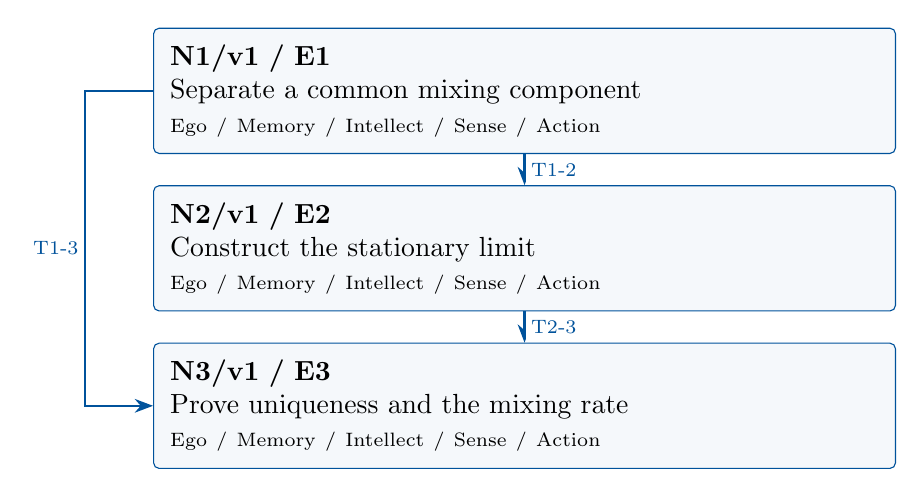
\begin{tikzpicture}[>=Stealth,x=1cm,y=1cm]

\node[mmnode,text width=9cm,minimum height=1.25cm] (N1) at (0,0.0) {\textbf{N1/v1 / E1}\\Separate a common mixing component\\{\scriptsize Ego / Memory / Intellect / Sense / Action}};

\node[mmnode,text width=9cm,minimum height=1.25cm] (N2) at (0,-2.0) {\textbf{N2/v1 / E2}\\Construct the stationary limit\\{\scriptsize Ego / Memory / Intellect / Sense / Action}};

\node[mmnode,text width=9cm,minimum height=1.25cm] (N3) at (0,-4.0) {\textbf{N3/v1 / E3}\\Prove uniqueness and the mixing rate\\{\scriptsize Ego / Memory / Intellect / Sense / Action}};

\draw[mmproof] (N1.south) -- node[mmnote,right] {T1-2} (N2.north);

\draw[mmproof] (N1.west) -- (-5.58,0) -- node[mmnote,left] {T1-3} (-5.58,-4) -- (N3.west);

\draw[mmproof] (N2.south) -- node[mmnote,right] {T2-3} (N3.north);

\end{tikzpicture}\end{center}

Each box is one mathematical agent containing all five faculties. Blue
arrows carry the versioned exports listed below. The layout gives a
reading order; only drawn arrows assert dependencies. Diagnostic repair
is separate from the proof DAG.

\subsection{Versioned evidence-transfer ledger}

\begingroup\small\linespread{1.05}\selectfont

\Needspace{5\baselineskip}\field{T1-2: N1/E1/v1 to N2}{If \(\delta<1\), \(P=\delta U+(1-\delta)Q\) for a stochastic \(Q\), and
\(\|\mu P-\nu P\|_1\le(1-\delta)\|\mu-\nu\|_1\).}

\field{Receiving activity}{N2.1}

\field{Compatibility}{E1/v1 with \(q=1-\delta\in[0,1)\) and \(\mu_n=\mu_0P^n\). Check:
Consecutive differences tending to zero is not enough; the summable
geometric tail provides the Cauchy property.}

\Needspace{5\baselineskip}\field{T1-3: N1/E1/v1 to N3}{If \(\delta<1\), \(P=\delta U+(1-\delta)Q\) for a stochastic \(Q\), and
\(\|\mu P-\nu P\|_1\le(1-\delta)\|\mu-\nu\|_1\).}

\field{Receiving activity}{N3.1}

\field{Compatibility}{E1/v1 and a stationary \(\pi\) from E2/v1. Check: The norm is on row
distributions, consistent with the stochastic convention; no column
convention is silently substituted.}

\Needspace{5\baselineskip}\field{T2-3: N2/E2/v1 to N3}{\(\mu_n\) converges to a probability vector \(\pi\) with \(\pi P=\pi\).}

\field{Receiving activity}{N3.1}

\field{Compatibility}{E1/v1 and a stationary \(\pi\) from E2/v1. Check: The norm is on row
distributions, consistent with the stochastic convention; no column
convention is silently substituted.}

\endgroup

\clearpage\section{Agent roles and five-faculty activities}\begingroup\small\linespread{1.05}\selectfont\setlist{itemsep=1pt,topsep=2pt}

\subsection{N1/v1: Separate a common mixing component}

\field{Object and role}{Write \(P\) as a convex combination of a uniform reset and a stochastic
residual. \textbf{Local obligation:} If \(\delta<1\),
\(P=\delta U+(1-\delta)Q\) for a stochastic \(Q\), and
\(\|\mu P-\nu P\|_1\le(1-\delta)\|\mu-\nu\|_1\).}

\field{Inputs}{\(\varepsilon>0\), \(\delta=d\varepsilon\), and the matrix \(U\) whose
every entry is \(1/d\).}

\mmfaculty{E}{Ego}{Publish E1/v1 only after establishing this obligation: If \(\delta<1\),
\(P=\delta U+(1-\delta)Q\) for a stochastic \(Q\), and
\(\|\mu P-\nu P\|_1\le(1-\delta)\|\mu-\nu\|_1\).}

\mmfaculty{M}{Memory}{\(\varepsilon>0\), \(\delta=d\varepsilon\), and the matrix \(U\) whose
every entry is \(1/d\). Retain the stated assumptions and import
versions.}

\mmfaculty{I}{Intellect}{Write \(P\) as a convex combination of a uniform reset and a stochastic
residual.}

\mmfaculty{S}{Sense}{The case \(\delta=1\) must be handled before dividing by \(1-\delta\).}

\mmfaculty{A}{Action}{Carry out activities N1.1--N1.2 below, retaining each calculation and
construction as evidence.}

\smallskip\noindent\textbf{Numbered mathematical activities}

\begin{enumerate}[label=N1.\arabic*,leftmargin=3.4em]

\item Row sums give \(d\varepsilon\le1\). If \(\delta=1\), every row entry
must equal \(1/d\), so \(P=U\). Otherwise define
\(Q_{ij}=(P_{ij}-\varepsilon)/(1-\delta)\). Its entries are nonnegative
and each row sums to one, proving the decomposition.

\item For any row vector \(z\),
\(\|zQ\|_1\le\sum_j\sum_i|z_i|Q_{ij}=\sum_i|z_i|=\|z\|_1\). For
probability vectors \(\mu,\nu\), \((\mu-\nu)U=0\), since their
coordinates both sum to one. The decomposition therefore gives the
contraction.

\end{enumerate}

\field{Export E1/v1}{If \(\delta<1\), \(P=\delta U+(1-\delta)Q\) for a stochastic \(Q\), and
\(\|\mu P-\nu P\|_1\le(1-\delta)\|\mu-\nu\|_1\).}

\field{Acceptance gate}{The case \(\delta=1\) must be handled before dividing by \(1-\delta\).}

\field{Targeted repair}{If strict positivity is replaced by nonnegativity, check whether
\(\varepsilon\) becomes zero; the strict contraction may then disappear.
Withhold this export and recheck its descendants after a versioned
correction.}

\clearpage

\subsection{N2/v1: Construct the stationary limit}

\field{Object and role}{Bound consecutive differences geometrically and sum the tail to prove
convergence inside the simplex. \textbf{Local obligation:} \(\mu_n\)
converges to a probability vector \(\pi\) with \(\pi P=\pi\).}

\field{Inputs}{E1/v1 with \(q=1-\delta\in[0,1)\) and \(\mu_n=\mu_0P^n\). Incoming proof
exports: E1/v1 at N2.1.}

\mmfaculty{E}{Ego}{Publish E2/v1 only after establishing this obligation: \(\mu_n\)
converges to a probability vector \(\pi\) with \(\pi P=\pi\).}

\mmfaculty{M}{Memory}{E1/v1 with \(q=1-\delta\in[0,1)\) and \(\mu_n=\mu_0P^n\). Incoming proof
exports: E1/v1 at N2.1. Retain the stated assumptions and import
versions.}

\mmfaculty{I}{Intellect}{Bound consecutive differences geometrically and sum the tail to prove
convergence inside the simplex.}

\mmfaculty{S}{Sense}{Consecutive differences tending to zero is not enough; the summable
geometric tail provides the Cauchy property.}

\mmfaculty{A}{Action}{Carry out activities N2.1--N2.2 below, retaining each calculation and
construction as evidence.}

\smallskip\noindent\textbf{Numbered mathematical activities}

\begin{enumerate}[label=N2.\arabic*,leftmargin=3.4em]

\item For \(q\in(0,1)\), contraction gives
\(\|\mu_{n+1}-\mu_n\|_1\le q^n\|\mu_1-\mu_0\|_1\). Therefore for
\(m>n\), \(\|\mu_m-\mu_n\|_1\le q^n\|\mu_1-\mu_0\|_1/(1-q)\). This tends
to zero uniformly in \(m>n\), so the sequence is Cauchy.

\item The simplex is closed in a complete finite-dimensional space, so the
limit \(\pi\) is a probability vector. Multiplication by \(P\) is
continuous; taking limits of \(\mu_{n+1}=\mu_nP\) yields stationarity.
If \(q=0\), \(P=U\) and every distribution becomes the uniform
distribution in one step, giving the same conclusion directly.

\end{enumerate}

\field{Export E2/v1}{\(\mu_n\) converges to a probability vector \(\pi\) with \(\pi P=\pi\).}

\field{Acceptance gate}{Consecutive differences tending to zero is not enough; the summable
geometric tail provides the Cauchy property.}

\field{Targeted repair}{If convergence is inferred from small single increments, insert the
displayed tail sum; it is the missing uniform bound over later indices.
Withhold this export and recheck its descendants after a versioned
correction.}

\clearpage

\subsection{N3/v1: Prove uniqueness and the mixing rate}

\field{Object and role}{Iterate the contraction against a fixed point and compare any two fixed
points. \textbf{Local obligation:} \(\pi\) is unique and the stated
geometric mixing estimate holds for all initial distributions.}

\field{Inputs}{E1/v1 and a stationary \(\pi\) from E2/v1. Incoming proof exports: E1/v1
at N3.1, E2/v1 at N3.1.}

\mmfaculty{E}{Ego}{Publish E3/v1 only after establishing this obligation: \(\pi\) is unique
and the stated geometric mixing estimate holds for all initial
distributions.}

\mmfaculty{M}{Memory}{E1/v1 and a stationary \(\pi\) from E2/v1. Incoming proof exports: E1/v1
at N3.1, E2/v1 at N3.1. Retain the stated assumptions and import
versions.}

\mmfaculty{I}{Intellect}{Iterate the contraction against a fixed point and compare any two fixed
points.}

\mmfaculty{S}{Sense}{The norm is on row distributions, consistent with the stochastic
convention; no column convention is silently substituted.}

\mmfaculty{A}{Action}{Carry out activities N3.1--N3.2 below, retaining each calculation and
construction as evidence.}

\smallskip\noindent\textbf{Numbered mathematical activities}

\begin{enumerate}[label=N3.\arabic*,leftmargin=3.4em]

\item If \(\pi'\) is another stationary distribution, contraction gives
\(\|\pi-\pi'\|_1\le q\|\pi-\pi'\|_1\). Since \(q<1\), the norm is zero,
proving uniqueness.

\item For any \(\mu\), repeatedly compare \(\mu P^n\) with \(\pi P^n=\pi\) to
obtain \(\|\mu P^n-\pi\|_1\le q^n\|\mu-\pi\|_1\). When \(q=0\) the
direct one-step conclusion applies. Thus existence, uniqueness, and the
quantitative rate are all established.

\end{enumerate}

\field{Export E3/v1}{\(\pi\) is unique and the stated geometric mixing estimate holds for all
initial distributions.}

\field{Acceptance gate}{The norm is on row distributions, consistent with the stochastic
convention; no column convention is silently substituted.}

\field{Targeted repair}{If existence of a stationary vector is assumed while proving
convergence, use E2's actual limit construction before invoking
stationarity in the estimate. Withhold this export and recheck its
descendants after a versioned correction.}

\endgroup\clearpage\section{Continuous mathematical proof}\label{sec:proof}

\subsection{N1 --- Separate a common mixing
component}\label{n1-separate-a-common-mixing-component}

\begin{enumerate}
\def\labelenumi{\arabic{enumi}.}
\item
  \textbf{N1.1.} Row sums give \(d\varepsilon\le1\). If \(\delta=1\),
  every row entry must equal \(1/d\), so \(P=U\). Otherwise define
  \(Q_{ij}=(P_{ij}-\varepsilon)/(1-\delta)\). Its entries are
  nonnegative and each row sums to one, proving the decomposition.
\item
  \textbf{N1.2.} For any row vector \(z\),
  \(\|zQ\|_1\le\sum_j\sum_i|z_i|Q_{ij}=\sum_i|z_i|=\|z\|_1\). For
  probability vectors \(\mu,\nu\), \((\mu-\nu)U=0\), since their
  coordinates both sum to one. The decomposition therefore gives the
  contraction.
\end{enumerate}

\subsection{N2 --- Construct the stationary
limit}\label{n2-construct-the-stationary-limit}

\begin{enumerate}
\def\labelenumi{\arabic{enumi}.}
\item
  \textbf{N2.1.} For \(q\in(0,1)\), contraction gives
  \(\|\mu_{n+1}-\mu_n\|_1\le q^n\|\mu_1-\mu_0\|_1\). Therefore for
  \(m>n\), \(\|\mu_m-\mu_n\|_1\le q^n\|\mu_1-\mu_0\|_1/(1-q)\). This
  tends to zero uniformly in \(m>n\), so the sequence is Cauchy.
\item
  \textbf{N2.2.} The simplex is closed in a complete finite-dimensional
  space, so the limit \(\pi\) is a probability vector. Multiplication by
  \(P\) is continuous; taking limits of \(\mu_{n+1}=\mu_nP\) yields
  stationarity. If \(q=0\), \(P=U\) and every distribution becomes the
  uniform distribution in one step, giving the same conclusion directly.
\end{enumerate}

\subsection{N3 --- Prove uniqueness and the mixing
rate}\label{n3-prove-uniqueness-and-the-mixing-rate}

\begin{enumerate}
\def\labelenumi{\arabic{enumi}.}
\item
  \textbf{N3.1.} If \(\pi'\) is another stationary distribution,
  contraction gives \(\|\pi-\pi'\|_1\le q\|\pi-\pi'\|_1\). Since
  \(q<1\), the norm is zero, proving uniqueness.
\item
  \textbf{N3.2.} For any \(\mu\), repeatedly compare \(\mu P^n\) with
  \(\pi P^n=\pi\) to obtain \(\|\mu P^n-\pi\|_1\le q^n\|\mu-\pi\|_1\).
  When \(q=0\) the direct one-step conclusion applies. Thus existence,
  uniqueness, and the quantitative rate are all established.
\end{enumerate}

\hfill$\square$

\section{Worked orchestration}

For
\(P=\bigl(\begin{smallmatrix}3/4&1/4\\1/2&1/2\end{smallmatrix}\bigr)\),
\(\varepsilon=1/4\), \(\delta=1/2\), and \(q=1/2\). Solving
\(\pi P=\pi\) gives \(\pi=(2/3,1/3)\). For \(\mu=(1,0)\), the initial
\(\ell^1\) distance is \(2/3\); after one step it is
\(|3/4-2/3|+|1/4-1/3|=1/6\le(1/2)(2/3)\).

\subsection{Boundary and hypothesis audit}

The nonnegative stochastic matrix
\(\bigl(\begin{smallmatrix}0&1\\1&0\end{smallmatrix}\bigr)\) has
stationary distribution \((1/2,1/2)\) but alternates forever from
\((1,0)\). Strict positivity is a sufficient mixing assumption here. It
is not necessary for all mixing chains, but dropping it without a
substitute invalidates this argument.

\section{Illustrative failure and repair}

The following is an authored diagnostic scenario. Changed assumptions
define a new contract; they do not retroactively prove the original
statement.

\subsection{Rejected argument, diagnosis, and correction}
\textbf{Rejected N2 claim:} every finite irreducible Markov chain
converges to stationarity. The two-state alternating chain is
irreducible but periodic. \textbf{Diagnosis:} Memory omitted the mixing
condition. \textbf{Repair:} use the strict-positive-entry contract,
which yields \(q<1\) directly. Recheck the geometric tail and the final
rate; a broader irreducible aperiodic theorem would need a separate
proof.

\subsection{Publication and reuse}
The corrected export retains its explicit assumptions. A hypothetical
revision receives a new version, and each consuming activity is
rechecked; this scenario is not a recorded runtime event. \textbf{Next
direction:} Extend the same method when a power \(P^m\) is strictly
positive, yielding mixing bounds in blocks of \(m\) steps.

\par\medskip\begingroup\small\linespread{1.0}\selectfont\noindent\textbf{Provenance.} This authored proof is complete relative to its declared imports. Reuse
each export with its assumptions, proof, and version. The original
Markdown remains available for comparison.
\par\endgroup

\par\smallskip\begingroup\small\linespread{1.0}\selectfont\noindent\textbf{Further reading.} \href{https://stanford.edu/~montanar/TEACHING/Stat310A/lnotes.pdf}{Amir
Dembo, Probability Theory: STAT310/MATH230 notes} for measure-theoretic
probability and limit arguments;
\href{https://web.stanford.edu/class/stats310c/syllabus.html}{Stanford
STAT310C syllabus and lecture materials} for martingale inequalities and
stopping theorems. The versions and proofs used in this collection are
stated explicitly.\par\endgroup

\end{document}
